\providecommand{\main}{..}
\documentclass[\main/main.tex]{subfiles}

\begin{document}

\lesson{12}{05/11/20}

\textbf{\textit{Summary}}:

Some keywords we have seen so far are:
\begin{itemize}
    \item \textbf{coupling}: the presence of a non-zero affinity which drives the system out-of-equilibrium implies that different observables respond to this non-zero affinity, non just the observable which is thermodynamically conjugated to that affinity;
    \item \textbf{linear response}: we are working always in the context of linear response i.e. the regime in which affinities are supposed to be small and we are dealing with phenomenological empirical laws;
    \item \textbf{non-equilibrium steady states (NESS)}: we are in a situation in which the system is in a stationary state but the entropy production rate is strictly positive.
\end{itemize}

\section{Coupled Transport in Linear Continuous Systems involving charged particles}

How we can revisit the following two empirical laws (which hold only in a LR regime), namely the 
\begin{itemize}
    \item \textbf{Fourier's law} for transport of heat: the energy/heat flux is just proportional to the temperature gradient $\vec{j}_u=-k\Vec{\nabla}T$ where $k$ is an example of transport coefficient and it's known as \textit{thermal conductivity}. 
    
    We can rewrite the Fourier's law using the Onsager formalism such that
    \begin{equation}
        \vec{j}_u=-\kappa\Vec{\nabla}T=\kappa T^2\Vec{\nabla}\left(\frac{1}{T}\right) \quad\left( \sim L_{uu}\mathbb{F}_u\right)
    \end{equation}
    where the gradient of $T^{-1}$ is the affinity of the system related to energy density.
    \item \textbf{Fick's law} for the particle current ($\rho$ is the number particles concentration) $\Vec{j}_\rho=-D\Vec{\nabla}\rho$ where the transport coefficient is the \textit{diffusion coefficient} $D$.
    
    We can rewrite the Fick's law using the Onsager formalism using the fact that in the context of a linear regime the concentration $\rho(\Vec{r})$ can be expressed as $\rho(\Vec{r}){=}\mu(\Vec{r})/T$\footnote{Actually the correct way to express the concentration is the following but when the difference in the equilibrium situation is small, $|\mu(\Vec{r})-\mu_0|<<1$:
    \[
    \rho(\Vec{r})=\rho_0 \exp{-\frac{\mu(\Vec{r})-\mu_0}{T}} \simeq \rho_0 - \left(1- \frac{\mu(\vec{r})-\mu_0)}{T}\right) \implies \rho(\Vec{r})\propto\mu(\Vec{r})/T 
    \]
    considering equilibrium averages equal to zero.
    }:
    \begin{equation}
        \Vec{j}_\rho=-D\Vec{\nabla}\rho=D\Vec{\nabla}\left(-\frac{\mu}{T}\right) \quad\left( \sim L_{\rho\rho}\mathbb{F}_\rho\right)
    \end{equation}
    where the affinity related to the concentration of particles is the gradient of $-\mu/T$.
\end{itemize}

Now we want to consider the situation of a continuous thermodynamic system made of a single species of particles contained in a fixed volume $V,$ where stationary energy and matter current densities are present at the same time. In this case the Gibbs relation for intensive observables specializes to:
$$
d u=T d s+\mu d \rho
$$
where $u, s,$ and $\rho$ are the densities of internal energy, entropy, and number of particles, respectively. Taking into account the previous phenomenological considerations, we can write the linear coupled transport equations (\ref{eq:combined}) in the form

\begin{align}
\vec{j}_{u} &=L_{u u} \vec{\nabla}\left(\frac{1}{T}\right)+L_{u \rho} \vec{\nabla}\left(\frac{-\mu}{T}\right) \\
\vec{j}_{\rho} &=L_{\rho u} \vec{\nabla}\left(\frac{1}{T}\right)+L_{\rho \rho} \vec{\nabla}\left(\frac{-\mu}{T}\right)
\end{align}

where $\vec{j}_{u}$ and $\vec{j}_{\rho}$ are the current densities. Note that, even if not explicitly indicated, all the physical quantities appearing in these equations are functions of the coordinate vector $\vec{r}$. The symmetric structure of Onsager matrix of linear coefficients yields the relation $L_{u \rho}=L_{\rho u},$ while the affinities are
\[
\vec{F}_{u} =\vec{\nabla}\left(\frac{1}{T}\right); \qquad
\vec{F}_{\rho} =\vec{\nabla}\left(\frac{-\mu}{T}\right)
\]
The entropy density production rate in the system is given then by the expression
\begin{equation}
  \frac{d s}{d t}=\vec{j}_{u} \cdot \vec{\nabla}\left(\frac{1}{T}\right)+\vec{j}_{\rho} \cdot \vec{\nabla}\left(\frac{-\mu}{T}\right)  
\end{equation}

We will use these equations to describe transport phenomena for charged particles, in particular in the presence of electric field (\textit{thermoelectric effect}): the presence of an electric field (and so of an electrostatic potential) implies that there are affinities related to the charged particle. 

\begin{appr}
We won't talk about the  \textit{magneto-thermoelectric effect} but let's state the \textit{Onsager theorem}, which takes into account the time-reversal properties that comes about in the presence of a magnetic field $\vec{B}$: \\

\textbf{Onsager theorem}: \textit{In the presence of a magnetic field $\vec{B}$ we can exchange the two indexes of the Onsager's coefficient provided the fact we reverse the direction of the magnetic field:}
\[
L_{ij}(\vec{B})=L_{ji}(-\vec{B})
\]
\end{appr}

\subsection{Thermoelectric effects}
These physical phenomena concern coupled transport of electric and heat currents \textbf{in the
absence of a magnetic field}. They result from the mutual interference of heat flow and
electric current. In this situation we are dealing with $1d$ metal/semiconductor wires and we adopt here the description of the conductor as a continuous system and
we specialize the Gibbs relation to:
\begin{equation}
    d s=\frac{1}{T} d u-\frac{\mu}{T} d n
\end{equation}
where $T$ is the temperature, $s$ is the local entropy density, $u$ is the local energy density,
$n$ is the number of electrons per unit volume (particle density), and, accordingly, $\mu$ is the chemical potential per particle.

The two relevant thermodynamical observables are $u$ and $n$, the affinities are $T^{-1}$ (related to the energy) and $-\mu/T$ (related to the particle density), while the equation for the current densities is:
\begin{equation}
    j_{s}=\frac{1}{T} j_{u}-\frac{\mu}{T} j_{n}
    \label{eq:above}
\end{equation}

Let's think about our particles as electrons, so the electric current is $ej_n$ (where $e<0$) and the entropy production rate can be written as:
\begin{equation}
    \frac{d s}{d t}=j_{u}\partial_{x}\left(\frac{1}{T}\right) - j_{n}\hlc{yellow}{\partial_{x}\left(\frac{\mu}{T}\right)}
\end{equation}
The point here is that it's not practical to deal with the yellow derivative because in general we would like to discuss a situation in which possibly both of the chemical potential and temperature depends on $x$: to solve this let's perform a 'change of variables' in which we switch from the energy flux\footnote{In $1d$ energy currents are actually fluxes because we don't have the area.} to the so called \textit{heat flux} $j_q$:
\begin{equation}
    j_u\mapsto j_q:=T j_s \overset{(\ref{eq:above})}{=} j_u-\mu j_n
    \label{eq:q_flux}
\end{equation}

We can now rewrite the EPR, separating the yellow gradient in two contributions and rearranging the terms together, as:
\begin{equation}
    \frac{d s}{d t}=j_{q}\partial_{x} \left(\frac{1}{T}\right) -\frac{j_{n}}{T}\partial_{x}\left( \mu\right) 
\end{equation}

so now we have the gradient of $T$ and $\mu$ split and the relevant quantities are heat and the number of particles.

In this way we can now rewrite the equation that uses that the Onsager matrix in the \textit{heat representation}\footnote{Energy is not equivalent to heat because we have a contribution from the electric field as we can see from (\ref{eq:q_flux}). We will discuss about how the electric fields enters in the chemical potential later.}:
\begin{equation}
\begin{aligned}
-j_{n} &=L_{n n} \frac{1}{T} \partial_{x} \mu+L_{n q} \partial_{x} \frac{1}{T} \qquad\qquad (a) \\
j_{q} &=L_{q n} \frac{1}{T} \partial_{x} \mu+L_{q q} \partial_{x} \frac{1}{T}\qquad \qquad (b)
\end{aligned}
\label{eq:heat_repr}
\end{equation}

The Onsager matrix is symmetric again because we don't have magnetic field ($L_{nq}=L_{qn}$) and now the interesting
question is how we relate the Onsager coefficients to physically relevant quantities (that can be measured)? What is the physical representation of the Onsager coefficients? \\

We have to deal with three independent coefficients: the two diagonal ones and the off-diagonal one, namely $L_{nn},L_{qq},L_{qn}$ and so we need three independent parameters that can be measured. 
\begin{enumerate}
    \item Let's start with a situation where the temperature is uniform ($\partial_xT=0$) and so we just have an electric field providing an electrostatic potential, which is varying along the wire, and an electric current.
    
    In this context we should call $\mu$ \textit{electrochemical potential} because it can be split in two different contributions, one taking into account the electrostatic potential and one coming from the chemical potential. In our context we are going to say that the actual chemical potential is zero because we are dealing with homogeneous materials
    \[
    \mu=\mu_e+\cancel{\mu_c}
    \]
    while the electrostatic potential component of the electrochemical potential is defined as:
    \[
    \mu_e=e\phi
    \]
    where $\phi$ is the actual electrostatic potential.
    
     On the other hand, $\mu_{c}$ is a function of $T$ and of the electronic concentration. In other words, the electrochemical potential per unit charge $(1 / e) \mu$ is such that its gradient $(1 / e) \partial_{x} \mu$ is the sum of the electric field $(1 / e) \partial_{x} \mu_{e}$ and of an effective driving force $(1 / e) \partial_{x} \mu_{c}$ associated with the presence of a concentration gradient of electrons. If we assume that the conductor is made of a homogeneous isothermal material, $\partial_{x} \mu_{c}=0$ and $\partial_{x} \mu=\partial_{x} \mu_{e},$ while the electric conductivity $\sigma$ is defined as the electric current density $e j_{n}$ per unit potential gradient $(1 / e) \partial_{x} \mu,$ i.e., the electromotive force. Thus the \textit{electric conductivity} is defined as the electric current density over the electric field:
    \begin{align}
            \sigma=\frac{e j_{n}}{-\partial_{x} \phi}=-\frac{e^{2} j_{n}}{\partial_{x} \mu}
    \end{align}
    For $\partial_{x} T=0$ (isothermal condition) using (\ref{eq:heat_repr}.a) the first diagonal Onsager coefficient is
    \begin{equation}
       \boxed{ L_{nn}=-\frac{Tj_n}{\partial_x \mu }=\frac{\sigma T}{e^2}}
       \label{eq:A}
    \end{equation}
    so in this way we got a first relation of one of the Onsager coefficients with the electric conductivity.
    
    Notice out that the definition of $\sigma$ is nothing but the Ohm's law.
    
    \item Now we want also to consider the Fourier's law: to consider this law let's consider the case in which $j_n=0$ (no electric currents flowing in the system, we just have energy or heat flux\footnote{In this case energy and heat flux are the same because $j_n=0$.}).
    
    The parameter we are interested in is the thermal conductivity $\kappa$ defined as:
    \begin{equation}
        \kappa=-\frac{j_q}{\partial_xT}
    \end{equation}
    
    Having constrain of $j_n=0$ in equation (\ref{eq:heat_repr}.a) tells us that:
    \begin{equation}
        \partial_x\mu=-T\frac{L_{nq}}{L_{nn}}\partial_x\left(\frac{1}{T}\right)=\frac{L_{nq}}{T L_{nn}}\partial_x T
        \label{eq:ref}
    \end{equation}
    while we can substitute the gradient of the electrochemical potential of the previous expression in equation (\ref{eq:heat_repr}.b)
    \begin{equation}
           j_q=\frac{1}{T^2}\frac{L^2_{nq}}{L_{nn}}\partial_x T=\frac{L_{qq}}{T^2}\partial_xT
    \end{equation} 
    and so we can rearrange this whole equation such that
    \begin{equation}
        j_q=\frac{1}{T^2}\frac{det(L)}{L_{nn}}\partial_xT
    \end{equation}
    
    Comparing this equation with the Fourier's law we can get a relation for the thermal conductivity as a function of the coefficients of the Onsager matrix:
    \begin{equation}
        \boxed{\kappa=\frac{det(L)}{T^2L_{nn}}}
        \label{eq:B}
    \end{equation}
 
    So far we got two equations (\ref{eq:A}) and (\ref{eq:B}) that allow us to relate the Onsager coefficients to physical quantities, such as the electric and thermal conductivity. We need a third one to finish. \\
    
    When we want to recover the Ohm's law we impose that there is no temperature gradient and equation (\ref{eq:A}) tells us that that the diagonal Onsager coefficient $L_{nn}$ is essentially the electric conductivity.
    
    On the other hand thermal conductivity involves all the coefficients in the Onsager matrix (through the determinant) because the presence of the off-diagonal Onsager coefficients, both in (\ref{eq:A}) and (\ref{eq:B}), tells us that in order to have zero current - since we have a non-diagonal Onsager coefficient - $L_{nq}$ in the first line of (\ref{eq:ref}), the presence of a temperature gradient would imply the flow of a current and in order to have zero current we need to have a gradient in the electrochemical potential. Here is where the coupling of transport phenomena comes in and this is essentially why at the end the thermal conductivity is actually depending on all the Onsager coefficients and not by $L_{qq}$ only. 
    
    \item In order to derive the third and last relation connecting the Onsager coefficient to physical parameters we need to consider tow peculiar effects due to the coupling between different affinities, the \textit{Seebeck effect} (1821) and the \textit{Peltier effect} (1834)
    \subsection{Seebeck effect}
    
    In the Seebeck effect we are dealing with two different kind of metals (e.g. Iron and Copper) or two differently doped semiconductors and with a \textit{temperature gradient} at the two junctions $T_2>T_1$: the solid line in Figure \ref{fig:Seebeck} represent one conductor ($A$ - Iron), while the lighter one the second ($B$ - Copper).
    
    \begin{figure}[ht]
        \centering
        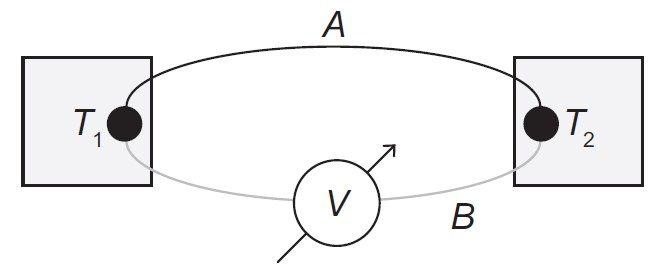
\includegraphics[width=0.7\linewidth]{Lectures/Images/seebeck.jpg}
        \caption{Sketch of the experimental apparatus to observe the Seebeck effect. Two different conducting (or semiconducting)
wires, $A$ and $B$, are joined at their ends (black dots), which are kept at different temperatures $T_1, T_2$. This temperature
gradient induces a difference of electric potential (electromotive force) at the inputs of the voltmeter $V$.}
        \label{fig:Seebeck}
    \end{figure}

We can have a setup in which we close the circuit (as represented in Figure \ref{fig:Seebeck}) and in this setup (without external electric fields initially) there is a so called \textit{thermoelectric power} for which a current flows in this circuit.

To discuss in detail the effect we will use the setup pf the \textit{thermocouple}: a thermocouple is a device that allows to measure temperature differences just reading the potential difference, so the actual instrument is a voltmeter\footnote{We assume the voltmeter to be \textbf{ideal}: no measurement perturbation and no current flowing $j_n=0$.}. 


\begin{appr}
The raw idea behind a thermocouple is that the voltage difference read in the voltmeter is related to the temperature difference between the two junctions.

The presence of the voltmeter is fundamental: is missing we have to deal with a \textit{stationary} current and with NESS which is surprising: we don't need an external field to maintain a constant current flowing in the circuit.
\end{appr}

In the thermocouple setup ($j_n=0$), in order to write fluxes as function of affinities using the Onsager coefficients, from equation (\ref{eq:heat_repr}.a) we get a relation between the variation of the electrochemical potential and the variation of temperature (going from $d(T^-1)\mapsto dT/T$ again):
\begin{equation}
    d \mu=\frac{L_{n q}}{T L_{n n}} d T
\end{equation}

Our aim is to compute the voltage measured by the voltmeter, where the index $r$ is referred to the point to the right of the voltmeter and $l$ the one to the left.

Let's compute the voltage\footnote{Sign convention: the point to the right has an higher voltage than the one to the left.} measured by the voltmeter. Integrating the previous expression over the two wires we can compute the electrochemical potential:
\begin{equation}
    \mu_r-\mu_l = \int_{\circled{1}}^{\circled{2}} \left[ \frac{L^A_{nq}}{L^A_{nn}} -\frac{L^B_{nq}}{L_{nn}^B}\right]\frac{dT}{T}
\end{equation}

Since we are dealing with different materials the values of the Onsager coefficients are different from each other while the '-' sign is due to the fact that we are integrating from the wire \circled{1} to the wire \circled{2}.

Finally, the measured voltage $V$ is given by the expression:
\begin{equation}
    V=\frac{\mu_r-\mu_l}{e}
\end{equation}

The\textit{(relative) thermoelectric power of a thermocouple}, $\varepsilon_{A B}$, is defined as the increment of voltage per unit temperature difference, while its sign is conventionally said to be positive if the increment of voltage drives the current from $A$ to $B$ at the hot junction, $T_{2} .$ In practice, if $T_{1}=T$ and $T_{2}=T+\Delta T,$ in the limit of small $\Delta T$

\begin{align}
    \varepsilon_{A B}:= \varepsilon_{B}-\varepsilon_{A}=\lim_{\Delta T\to 0}
    \underbrace{\frac{\mu_r-\mu_l}{e}}_{\text{V}} \frac{1}{\Delta T} 
\end{align}


In practise the effect can be measured only when you join two different conductors and practically we will always measure the relative power coming from the different properties of the two conductors materials but it is useful to define the coefficient 

\begin{equation}
    \boxed{\varepsilon_{X}=-\frac{L_{n q}^{X}}{e T L_{n n}^{X}}, \quad X=A, B}
    \label{eq:c}
\end{equation}

which defines the\textit{ absolute thermoelectric power} of a single electric conductor and is our last relation. Equation (\ref{eq:c}) is the third relation that we needed to express all coefficients of Onsager matrix using physically measurable quantities. \\

Considering the definition we gave of absolute thermoelectric powers and we compare it to the  way we expressed the electrochemical potential difference then in the limit of $\Delta T\to 0$ we can get rid of the integral and we can read the definition of absolute thermoelectric power from the argument of the integral. 
\end{enumerate}

Let's now rearrange (\ref{eq:A}), (\ref{eq:B}), (\ref{eq:c}):
\begin{equation}
    L_{nn}\overset{(\ref{eq:A})}{=}\frac{T\sigma}{e^2}; \quad L_{nq}=L_{qn}\overset{(\ref{eq:c})}{=}-\varepsilon eTL_{nn}\overset{(\ref{eq:A})}{=}\frac{-T^2\sigma\varepsilon}{e}
\end{equation}
 where the last relation holds for any material.
 now our aim is to explicitly write each of the Onsager coefficients as a function of $\sigma,\kappa,\varepsilon$. 
 
 From equation (\ref{eq:B}) we get that:
 \begin{equation}
     L_{qq}=\kappa T^2 + \varepsilon^2\sigma T^3
 \end{equation}
 
and so eventually we can rewrite the coupled transport equation expressing the Onsager coefficients in this way, in order to read immediately the physically relevant parameters:

\begin{equation}
\begin{aligned}
(a) \qquad \,\,\,\, -j_{n} &=\left(\frac{\sigma}{e^{2}}\right) \partial_{x} \mu-\left(\frac{T^{2} \sigma \varepsilon}{e}\right) \partial_{x} \frac{1}{T} \qquad \qquad  \\
(b) \qquad \qquad j_{q} &=-\left(\frac{T^2 \sigma \varepsilon}{e}\right) \partial_{x} \mu+\left(T^{3} \sigma \varepsilon^{2}+T^{2} \kappa\right) \partial_{x} \frac{1}{T}
\label{eq:nuovo}
\end{aligned}
\end{equation}

This is everything we need to know to describe all possible phenomena related to coupled transport of heat and electricity current. \\

For example, taking into account (\ref{eq:nuovo}.a), the electric field is zero the first term is missing and we can see that - thanks to the Seebeck effect ($\varepsilon$ is present) - we observe a particle flux/current due to a temperature gradient.

On the other hand, if $j_n=0$ we can observe a voltage difference related to the presence of a temperature gradient. \\

Noticing out that the first two terms of (\ref{eq:nuovo}).b are proportional to the particle current let's rewrite the heat flux $j_q$ such that:
\begin{equation}
    j_q=T\varepsilon e j_n + \kappa T^2\partial_x \left(\frac{1}{T}\right)
\end{equation}
which is a more transparent way because we isolate the contribution from thermal conductivity and then we can see that the Seebeck contribution $\varepsilon$ is really related to the fact that an electric current $j_n$ is coupled to an heat current.

This allows us to provide this expression (remembering that the heat current is proportional to the entropy current):
\begin{equation}
    j_{s}=\frac{j_q}{T}=\varepsilon e j_{n}+T \kappa \partial_{x} \frac{1}{T}
\end{equation}
which is a clear interpretation of what it's going on: entropy is produced by  a temperature gradient through a thermal conductivity (Fourier's law) but then if we have charged particles moving they carry with themselves entropy and we can reinterpret $\varepsilon$ as the \textit{entropy transported per unit charge}. If a charged particle is moving, is carrying some entropy.

\subsection{Peltier effect}
We can think of the Peltier effect as a 'reversed Seebeck': in this setup we have one junction (between two different conductors) at constant temperature $T$. The solid line of Figure \ref{fig:peltier} represent conductor A, while the lighter one conductor B.

In the Seebeck effect, in the thermopower setup, a heat flows implies a heat current; here it's reversed in the sense that it's the other way round and what's happening is that we have a discontinuity in the electric current at the junction due to the fact that we are dealing with two different materials and this is implying a discontinuity also in the heat fluxes. For instance, in a situation like this (where the arrows in Figure \ref{fig:peltier} refer to heat currents), energy needs to be conserved, so if the the currents are higher in B than in A and are flowing in the direction showed in Figure \ref{fig:peltier} what happens is that heat is released from the junction to the system: the discontinuity due to the junction implies that heat needs to be transferred to the system and this effect is used in heaters/heat pumps for this reason. 

\begin{figure}[ht]
    \centering
    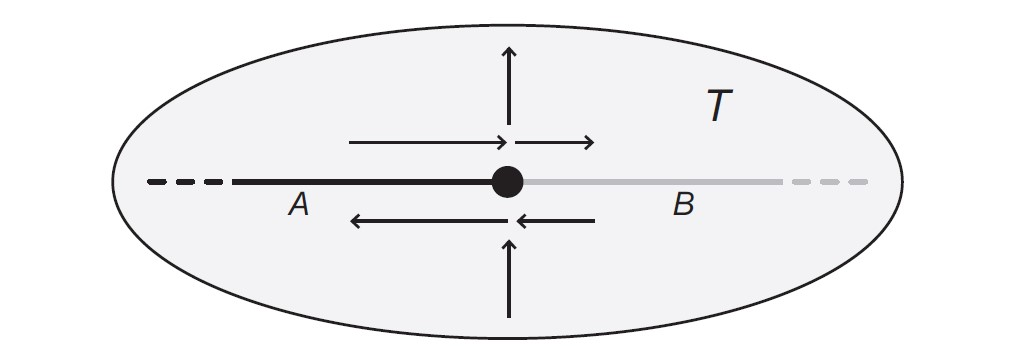
\includegraphics[width=0.7\linewidth]{Lectures/Images/peltier.jpg}
    \caption{The diagram of the Peltier effect. A junction (black dot) of two different conductors A and B, when kept at constant temperature T, must exchange heat with the reservoir in order to sustain a constant electric current. The horizontal arrows correspond to $j_q^A$ and $j_q^B$: their difference amounts to the heat exchanged with the environment at temperature $T$, which may be either positive or negative; see the two cases above and below the junction.}
    \label{fig:peltier}
\end{figure}

A different situation can be presented when we reverse the direction of the currents (top arrows in Figure \ref{fig:peltier}) and in this case we need to \textit{absorbed} heat into the junction in order to conserve energy: this is a way to extract heat from the environment and this setup is used for refrigerators. \\

Let's consider the heater setup: it's very different from the \textit{Joule effect} because the Peltier effect is due to the presence of a junction and the heat can be either taken or absorbed by the junction and we can control whether it's a heater or a cooler.

In this setup we are in a situation where temperature is constant ($\partial_x T=0$) and therefore, using (\ref{eq:nuovo}.a) for the particle flux:
\begin{equation}
    j_n=-\frac{\sigma}{e^2}\partial_x\mu
\end{equation}
while using (\ref{eq:nuovo}.b) for the heat flux:

\begin{equation}
    j_q=-\frac{T\sigma\varepsilon}{e}\partial_x\mu
\end{equation}
Considering the ratio between the two previous equations we get that the heat flux is proportional to the electric current:
\begin{align}
    j_q=T\varepsilon \,\,\,\, \cdot \underbrace{(e j_n)}_{\text{electric current}}
\end{align}

From the Seebeck effect we have learnt that for two different materials $\varepsilon$ is different which implies that at the junction we have a discontinuity in the heat flux:
\begin{equation}
    j_q^B-j_q^A=T(\varepsilon_B-\varepsilon_A)(e j_n)
    \label{eq:disco}
\end{equation}
So the electric current is \textbf{continuous} but the discontinuity arises because the Seebeck coefficients $\varepsilon$ are different (due to the presence of a junction) and therefore we have a discontinuity in the heat flux, as described by (\ref{eq:disco}). \\

We can quantify the effect defining the \textit{Peltier coefficients} $\Pi_{AB}$
\begin{equation}
    \boxed{\Pi_{A B}:=T\left(\varepsilon_{B}-\varepsilon_{A}\right)}
\end{equation}
which is the heat supplied to the junction per unit electric current (as we can read from (\ref{eq:disco})).

The sign convention in this case is such that positive ($\Pi_{AB}>0$) means that heat is supplied to the junction. \\

Let's now assume that $\varepsilon_B>\varepsilon_A$ and let's discuss the two possible situation (heater/cooler setup):
\begin{itemize}
\item \textit{Heater setup}: if $j_n>0$ then electrons are flowing from left to right and so current (remember that $e<0$) and therefore the heat flux (which is proportional to the current through a positive Peltier coefficient) are instead negative: $ej_n,j_q<0$ and $j_q^B<j_q^A$ consistently with the bottom sketch of Figure \ref{fig:peltier};
\item \textit{Cooler setup}: if $j_n<0$ then electrons are flowing from right to left and so current (remember that $e<0$) and therefore the heat flux (which is proportional to the current through a positive Peltier coefficient) are instead positive: $ej_n,j_q>0$ and $j_q^B>j_q^A$ consistently with the bottom sketch of Figure \ref{fig:peltier}.
\end{itemize}

See Chapter \ref{thomson}, Appendix B for more details.


\end{document}